\chapter{Implementação}\label{CapImpl}

%\resumodocapitulo{Resumo opcional}

\section{Caminho de Dados}
{
    O caminho de dados projetado para a implementação da microarquitetura
    uniciclo é apresentado na Figura~\ref{fig:datapath}.
}

\begin{figure}[H]
\centering
    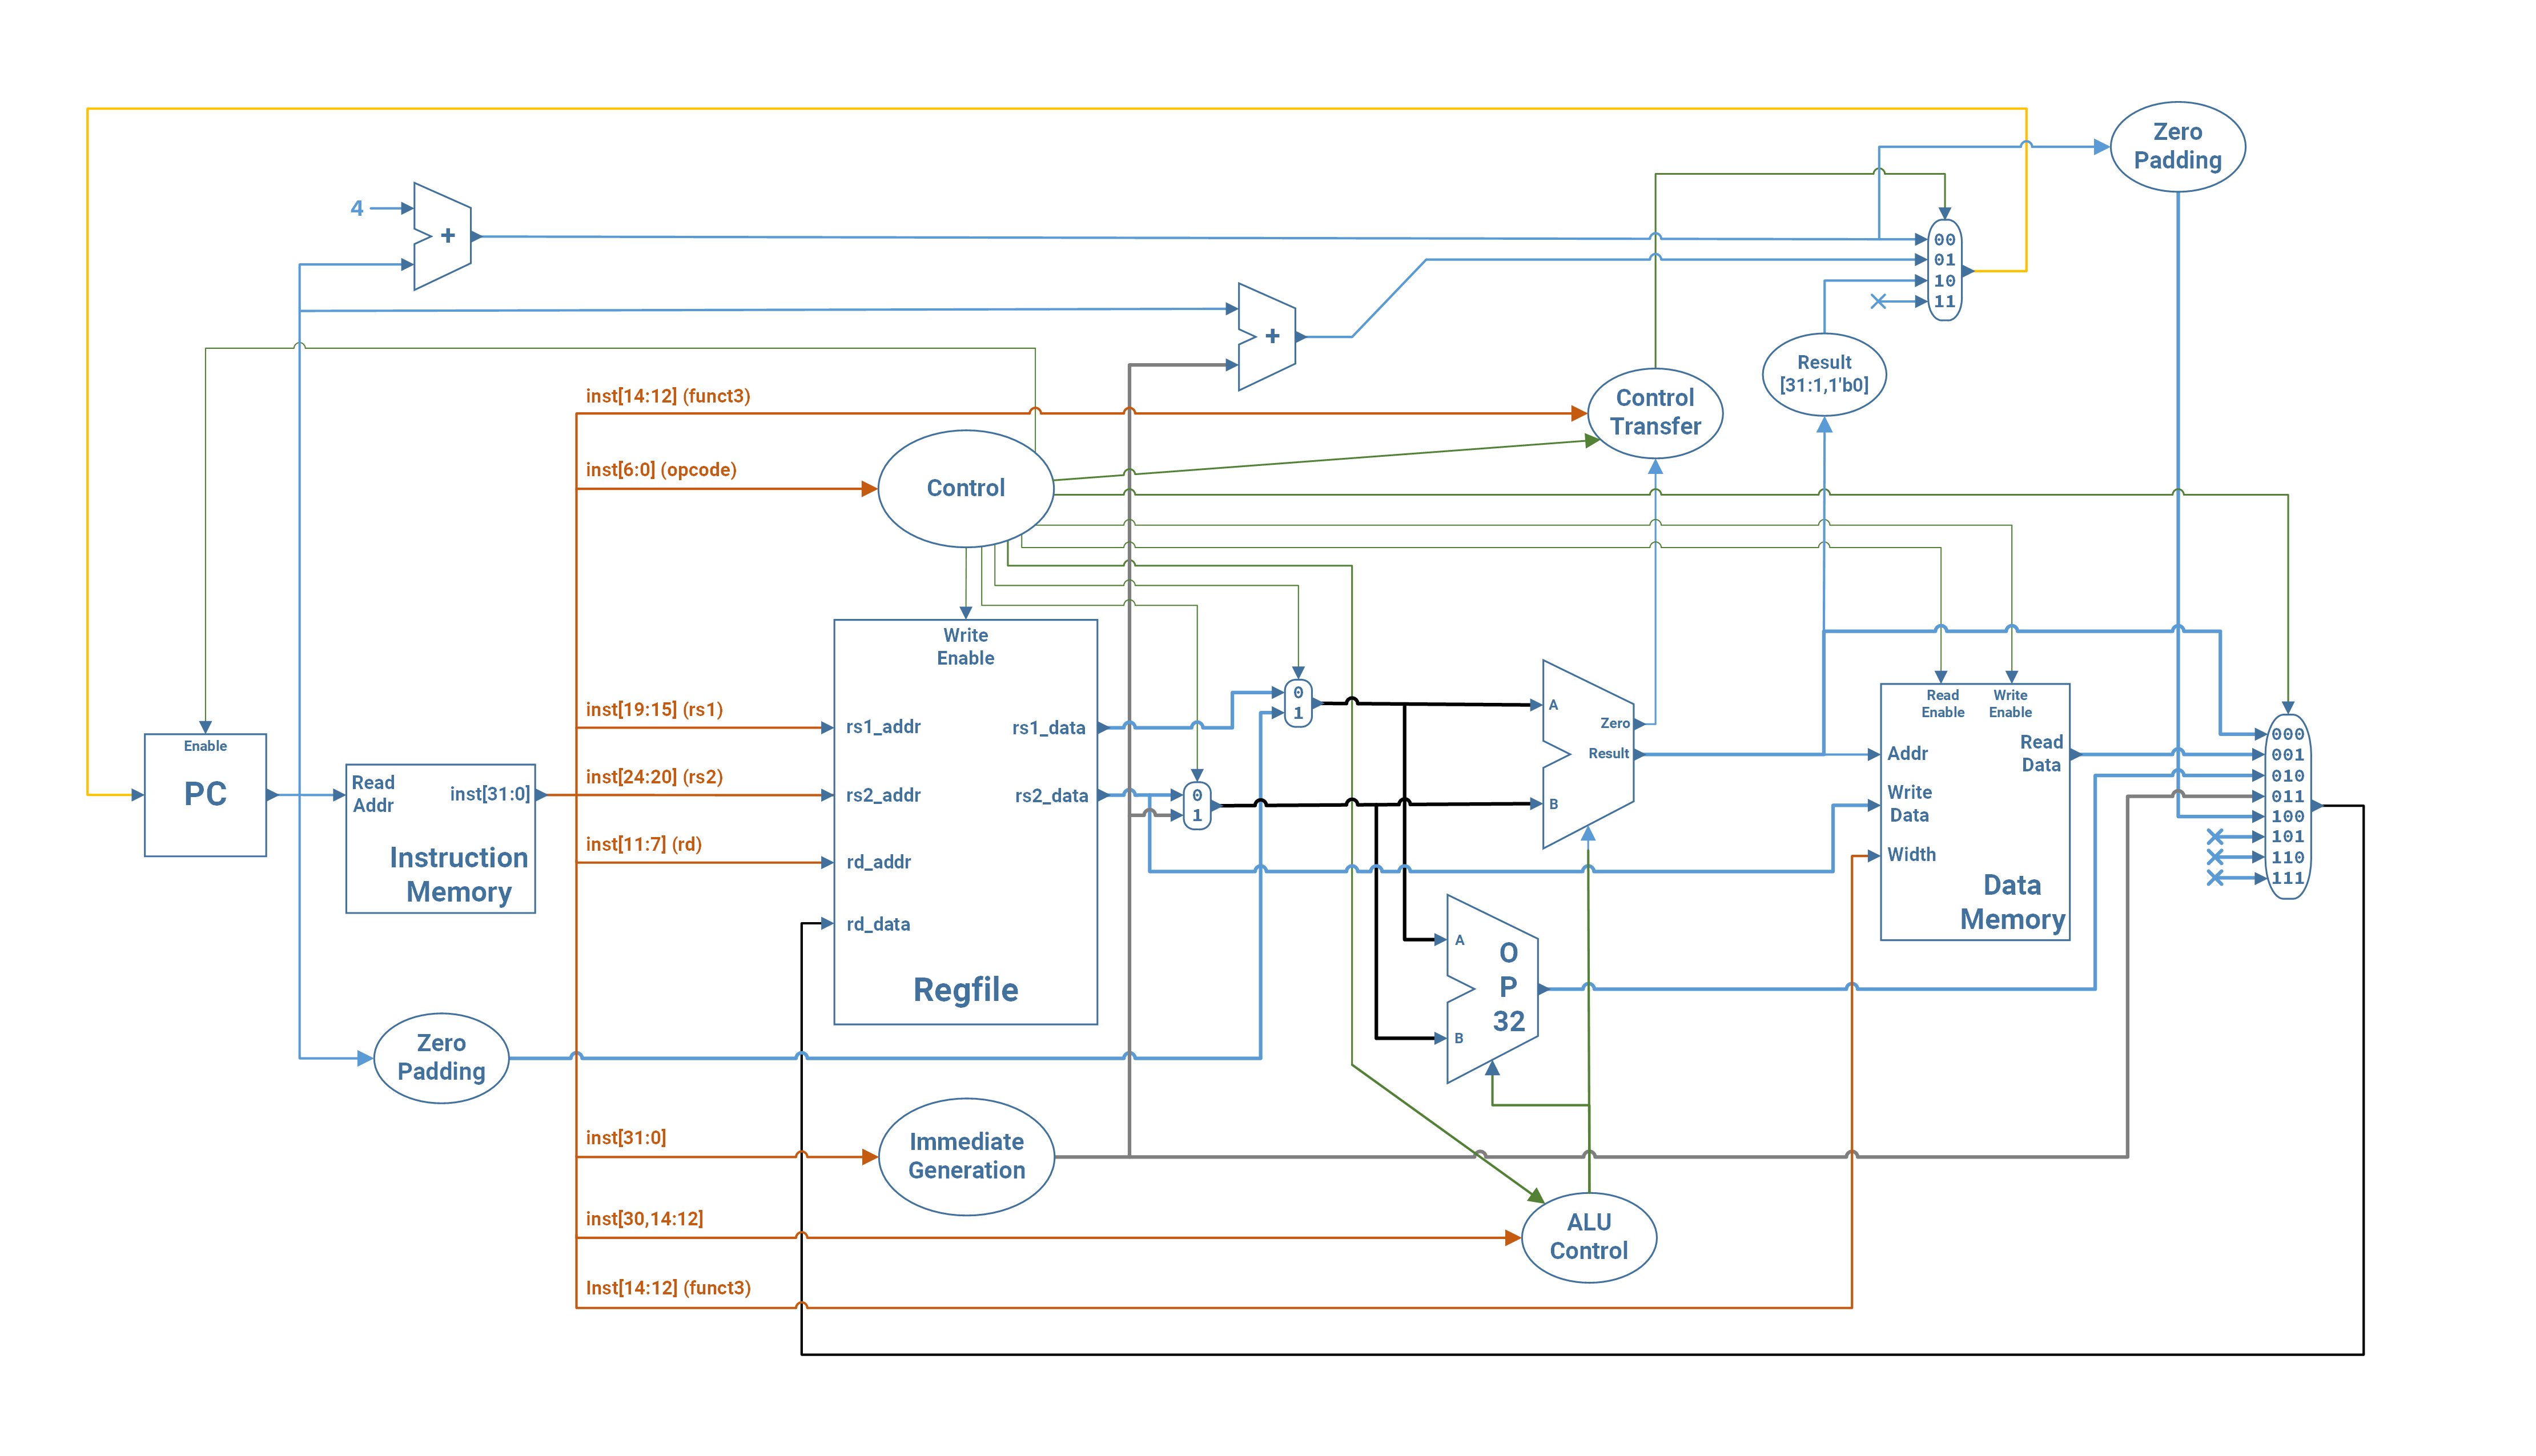
\includegraphics[width=1\linewidth]{images/singlecycle.png}
    \caption{Caminho de Dados implementado para o
                módulo I}\label{fig:datapath}
\end{figure}

{
    O \textit{datapath} possui um banco de 32 registradores de uso geral
    de 64 bits cada. A memória possui arquitetura Harvard, sendo a memória
    de instruções (\textit{text}) \textit{read-only} e a memória de dados
    (\textit{data}) \textit{read-write}.
    São implementadas 49 instruções, sendo elas:
}

\begin{itemize}[leftmargin=20mm]
    \item {LUI:\@ Load Upper Intermediate;}
    \item {AUIPC:\@ Add Upper Intermediate to Program Counter;}
    \item {JAL:\@ Jump And Link;}
    \item {JALR:\@ Jump And Link Register;}
    \item {BEQ:\@ Branch if EQual;}
    \item {BNE:\@ Branch if Not Equal;}
    \item {BLT:\@ Branch if Less Than;}
    \item {BGE:\@ Branch if Greater or Equal;}
    \item {BLTU:\@ Branch if Less Than Unsigned;}
    \item {BGEU:\@ Branch if Greater or Equal Unsigned;}
    \item {LB:\@ Load Byte;}
    \item {LH:\@ Load Halfword;}
    \item {LW:\@ Load Word;}
    \item {LBU:\@ Load Byte Unsigned;}
    \item {LHU:\@ Load Halfword Unsigned;}
    \item {SB:\@ Store Byte;}
    \item {SH:\@ Store Halfword;}
    \item {SW:\@ Store Word;}
    \item {ADDI:\@ ADD Immediate;}
    \item {SLTI:\@ Set on Less Than;}
    \item {SLTIU:\@ Set on Less Than Unsigned;}
    \item {XORI:\@ XOR Immediate;}
    \item {ORI:\@ OR Immediate;}
    \item {ANDI:\@ AND Immediate;}
    \item {SLLI:\@ Shift Left Logical Immedate;}
    \item {SRLI:\@ Shift Right Logical Immediate;}
    \item {SRAI:\@ Shift Right Arithmetic Immediate;}
    \item {ADD:\@ ADD;}
    \item {SUB:\@ SUB;}
    \item {SLL:\@ Shift Left Logical;}
    \item {SLT:\@ Set on Less Than;}
    \item {SLTU:\@ Set on Less Than Unsigned;}
    \item {XOR:\@ XOR;}
    \item {SRL:\@ Shift Right Logical;}
    \item {SRA:\@ Shift Right Arithmetic;}
    \item {OR:\@ OR;}
    \item {AND:\@ AND;}
    \item {LWU:\@ Load Word Unsigned;}
    \item {LD:\@ Load Double;}
    \item {SD:\@ Store Double;}
    \item {ADDIW:\@ ADD Immediate Word-size;}
    \item {SLLIW:\@ Shift Left Logical Immedate Word-size;}
    \item {SRLIW:\@ Shift Right Logical Immediate Word-size;}
    \item {SRAIW:\@ Shift Right Arithmetic Immediate Word-size;}
    \item {ADDW:\@ ADD Word-size;}
    \item {SUBW:\@ SUB Word-size;}
    \item {SLLW:\@ Shift Left Logical Word-size;}
    \item {SRLW:\@ Shift Right Logical Word-size;}
    \item {SRAW:\@ Shift Right Arithmetic Word-size;}
\end{itemize}

{
    Para que o processador seja completamente compatível com a
    especificação da \textit{ISA}, falta implementar tratamentos de
    exceções, interrupções e \textit{traps}, Registradores \textit{CSR},
    instruções de chamada ao ambiente (ECALL/EBREAK), instruções de
    \textit{fencing} de memória, suporte ao acesso desalinhado à memória
    de dados e pilha de endereço de retorno (RAS).
}

\section{\textit{Hardware Description Language}}
{
    Linguagens de Descrição de Hardware, ou \textit{HDL's} são linguagens de
    programação que permitem a descrição em alto nível de um circuito lógico.
}

{
    Diferente de diagramas de blocos onde se descreve o circuito a nível de
    portas lógicas, em uma \textit{HDL} o comportamento do circuito é descrito
    por funções, e um sintetizador de \textit{hardware} (programa similar a um 
    compilador) transforma as funções em circuitos.
}

{
    O uso de \textit{HDL's} possui muitas vantagens em relação aos diagramas de
    blocos. Por se tratar de uma linguagem com maior nível de abstração, o
    entendimento das lógicas de funcionamento se um circuito são mais fáceis de
    se entender, alem de permitir o uso de sistemas de versionamento de código
    e.g.\ git para manter um histórico de todas as alterações feitas.
}

{
    O código a seguir foi retirado do módulo de transferência de controle do 
    processador e exemplifica a estrutura de um programa em Verilog, a 
    linguagem de descrição de \textit{hardware} utilizada no projeto:
}

\begin{lstlisting}[style={verilog-style}]
module control_transfer_singlecycle (
    input  branch_en,
    input  jal_en,
    input  jalr_en,
    input  result_eq_zero,
    input  [2:0] inst_funct3,

    output reg [1:0] pc_sel
);

always @ ( * ) begin
    if (branch_en) begin
        case (inst_funct3)
            `BRANCH_EQ:
                pc_sel = result_eq_zero ? 2'b01 : 2'b00;

            `BRANCH_NE:
                pc_sel = result_eq_zero ? 2'b00 : 2'b01;

            `BRANCH_LT:
                pc_sel = result_eq_zero ? 2'b00 : 2'b01;

            `BRANCH_GE:
                pc_sel = result_eq_zero ? 2'b01 : 2'b00;

            `BRANCH_LTU:
                pc_sel = result_eq_zero ? 2'b00 : 2'b01;

            `BRANCH_GEU:
                pc_sel = result_eq_zero ? 2'b01 : 2'b00;

            default:
                pc_sel = 2'b00;
        endcase
    end

    else if (jal_en) begin
        pc_sel = 2'b01;
    end

    else if (jalr_en) begin
        pc_sel = 2'b10;
    end

    else begin
        pc_sel = 2'b00;
    end
end

endmodule

\end{lstlisting}

\section{\textit{Field Programmable Gate Array}}
{
    As \textit{FPGA's} são circuitos integrados que possuem uma matriz de
    blocos lógicos configuráveis. Um diagrama de blocos ou uma \textit{HDL},
    após passar pelo processo de síntese (transformação em uma linguagem
    intermediária que representa o circuito a nível \textit{TTL}) passa pelos
    processos de mapeamento e alocação (\textit{mapping} e \textit{fitting})
    que conectam os elementos da matriz. Assim, o código ou diagrama são
    ``traduzidos'' em um circuito.
}

\begin{figure}[H]
\centering
    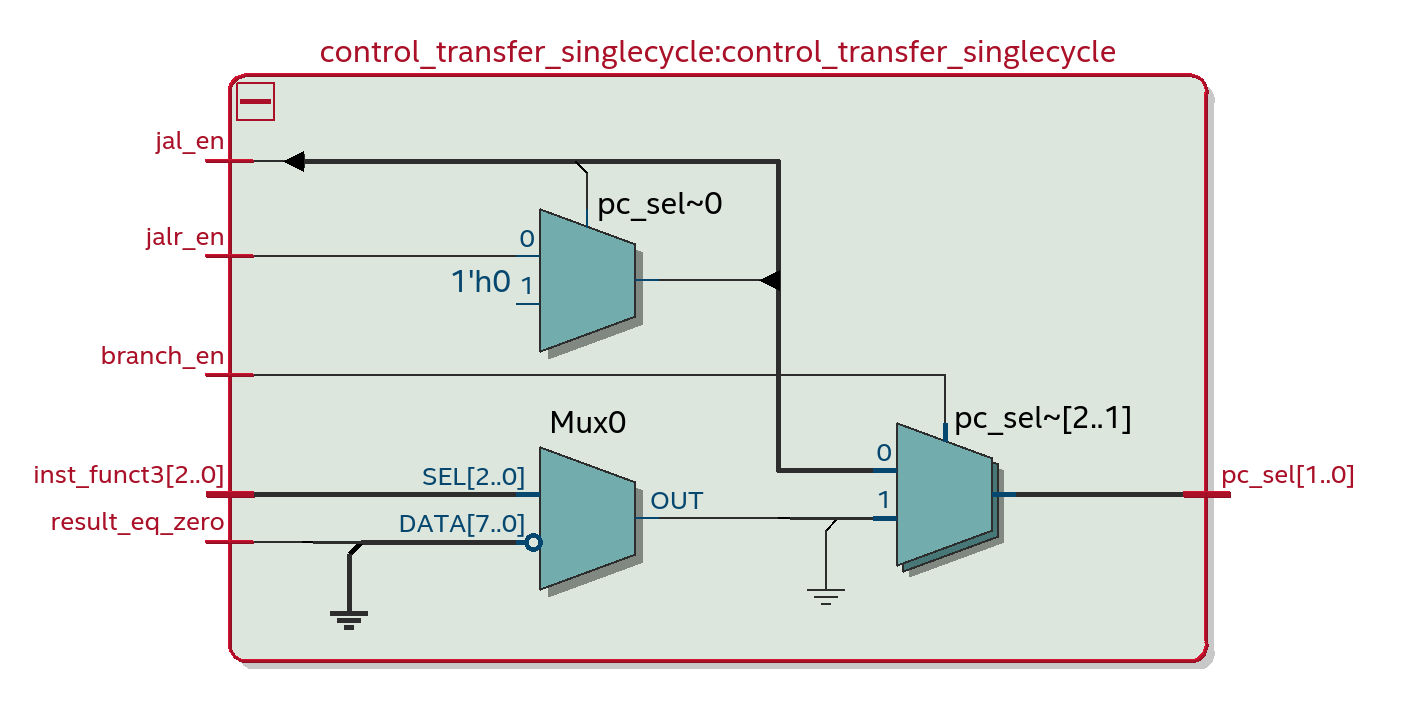
\includegraphics[width=1\linewidth]{images/riscv_sinth.png}
    \caption{Módulo de Transferência de Controle após ser sintetizado
                }\label{fig:riscv_sinth}
\end{figure}

{
    \textit{Kits} de desenvolvimento possuem, além da \textit{FPGA}, diversos
    periféricos conectados a ela, permitindo interfacear o circuito sinteitzado
    com saídas de vídeo, portas USB, memórias FLASH, entre outros componentes.
    A Figura~\ref{fig:DE2_115} apresenta a placa de desenvolvimento DE2-115
    produzida pela empresa \textit{terasIC}.
}

\begin{figure}[H]
\centering
    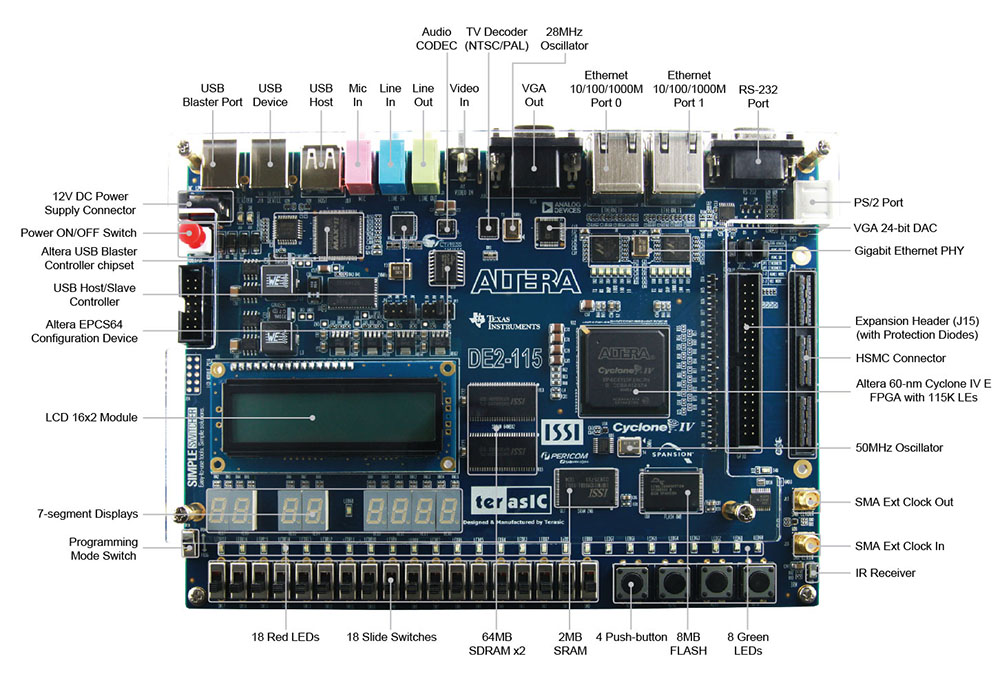
\includegraphics[width=1\linewidth]{images/DE2_115.jpg}
    \caption{Placa de desenvolvimento DE2-115 da terasIC
                }\label{fig:DE2_115}
\end{figure}

